\providecommand{\zZ}{\hskip 3.6pt plus1.2pt minus0.8pt}
\providecommand{\McQ}{\fontfamily{cwM}\fontseries{2}\selectfont}
\providecommand{\MbQ}{\fontfamily{cwM}\fontseries{1}\selectfont}
\providecommand{\zz}{\hskip 0.6pt plus0.2pt minus0.1pt\ignorespaces}
\providecommand{\MdQ}{\fontfamily{cwM}\fontseries{3}\selectfont}
\catcode+252=1 \catcode+253=2 \catcode+254=0 \catcode+251=4
\providecommand{\MmQ}{\fontfamily{cwM}\fontseries{12}\selectfont}
\providecommand{\z}{\hskip 0.0pt plus0.2pt minus0.1pt}
\providecommand{\Z}{\hskip 1.2pt plus0.4pt minus0.2pt}
\providecommand{\cH}{\char}
\providecommand{\MjQ}{\fontfamily{cwM}\fontseries{9}\selectfont}
\documentclass[a4paper,12pt]{article}
\usepackage{ amssymb }
\usepackage{ stmaryrd }
\usepackage{ dsfont }
\usepackage{amsmath}
\usepackage{mathtools} 
\newcommand{\tabincell}[2]{\begin{tabular}{@{}#1@{}}#2\end{tabular}} %{\McQ\cH91}{\MbQ\cH143}{\MaQ\cH113}{\MbQ\cH35}{\MaQ\cH132}{\MfQ\cH178}{\McQ\cH87}{\MaQ\cH223}{\MbQ\cH224}
\usepackage{textcomp}
\renewcommand{\baselinestretch}{1.5} % 5 linespace
%\usepackage{MinionPro} %{\MiQ\cH28}{\MfQ\cH220}{\MiQ\cH116}{\MbQ\cH143}{\MbQ\cH61}{\MbQ\cH224}{\MbQ\cH237}{\McQ\cH76}{\MbQ\cH100}{\MbQ\cH98}{\MaQ\cH229}{\MaQ\cH229}{\McQ\cH241}
\usepackage[utf8]{inputenc}
\usepackage{geometry}
\usepackage{graphicx,psfrag,booktabs}
\geometry{left=1in,right=1in,top=1in,bottom=1in}
\usepackage{graphicx}
\usepackage{titlesec}
\titlelabel{\thetitle.\quad} %{\MaQ\cH94}{\MbQ\cH90}section {\McQ\cH41}{\McQ\cH85}{\MbQ\cH237}{\MeQ\cH165}{\MdQ\cH168}
\usepackage{mathrsfs} %{\MaQ\cH139}{\MaQ\cH112}{\McQ\cH73}{\McQ\cH241}{\MaQ\cH229}{\MgQ\cH130}{\MeQ\cH165}{\MdQ\cH168}
%\usepackage{indentfirst}%{\McQ\cH199}{\McQ\cH229}{\McQ\cH11}{\MaQ\cH115}{\MbQ\cH143}{\MbQ\cH237}{\MbQ\cH78}{\MaQ\cH73}
\usepackage[square,numbers]{natbib}
\usepackage{xeCJK} %{\MaQ\cH50}{\MbQ\cH100}{\MaQ\cH229}{\McQ\cH241}{\McQ\cH113}{\MaQ\cH236}
\setCJKmainfont{SimSun} %{\McQ\cH227}{\McQ\cH113}{\MaQ\cH53}{\MaQ\cH50}{\MbQ\cH100}{\MaQ\cH229}{\McQ\cH241}
\bibliographystyle{unsrtnat}
\makeatletter
\def\@xfootnote[#1]{%
  \protected@xdef\@thefnmark{#1}%
  \@footnotemark\@footnotetext}
\makeatother

\title{Home Work 4\\ Machine Learning Foundations}
\author{R04323050 \\{\McQ\cH37}\z{\MbQ\cH200}\z{\MmQ\cH238}\z{\McQ\cH250}   \quad {\McQ\cH207}\z{\MdQ\cH43}\z{\MjQ\cH254}}
\date{}

\begin{document}
\maketitle
\section{}
\begin{figure}[h]
\centering

\includegraphics[scale=0.38]{Q1.png}
\end{figure}

\newpage

\section{}
$\displaystyle E_{aug}(\mathbf{w})=E_{in}(\mathbf{w})+ \frac{\lambda}{N} \mathbf{w}^{T} \mathbf{w}$ \\
Take the derivatives of $\displaystyle \mathbf{w}$: $\nabla E_{aug}(\mathbf{w})= \nabla E_{in}(\mathbf{w}) + \frac{2 \lambda}{N} \mathbf{w}$ \\
By the Gradient Descent: 
\begin{align*} 
 \mathbf{w}_{t+1} \leftarrow &\mathbf{w}_{t} - \eta \cdot (\nabla E_{aug}(\mathbf{w})) \\
  &= \mathbf{w}_{t} - \eta \cdot (\nabla E_{in}(\mathbf{w}_{t}) + \frac{2 \lambda}{N} \mathbf{w}_{t}) \\
  &= (1- \frac{2 \eta \lambda}{N}) \mathbf{w}_{t} - \eta \nabla E_{in}(\mathbf{w}_{t})
\end{align*}

\section {}
Regularized Regression Problem:
\begin{align*} 
  \min_{\mathbf{w}}  \quad E_{in}(\mathbf{w})= \mathbf{\frac{1}{N} (Zw-y)^{T} (Zw-y)   } \quad \quad
   \text{s.t.} \quad \mathbf{ w^T w } \leq C
\end{align*}
\textcircled{1} If $\mathbf{w}_{lin}$ satisfies the constraints $ \; \mathbf{ w^T w } \leq C$, then $\mathbf{w}_{reg}$ is equivalent to $\mathbf{w}_{lin}$, thus $\left \| \mathbf{w}_{reg} \right \| = \left \| \mathbf{w}_{lin} \right \|$. \\
\textcircled{2} If $\mathbf{w}_{lin}$ does not satisfy the constraints $\quad \mathbf{ w^T w } \leq C$, which means $\left \| \mathbf{w}_{lin} \right \|^2 > C$; on the other hand, we know $\mathbf{w}_{reg}$ satisfies the constraints, i.e $\left \| \mathbf{w}_{reg} \right \|^2 \leq C$. Hence, $\left \| \mathbf{w}_{reg} \right \| < \left \| \mathbf{w}_{lin} \right \|$.\\
By \textcircled{1}{\MaQ\cH2}\textcircled{2}, we have $\left \| \mathbf{w}_{reg}(\lambda) \right \| \leq \left \| \mathbf{w}_{lin} \right \|$ for all $\lambda > 0$.


\section{}
\begin{figure}[h]
\centering
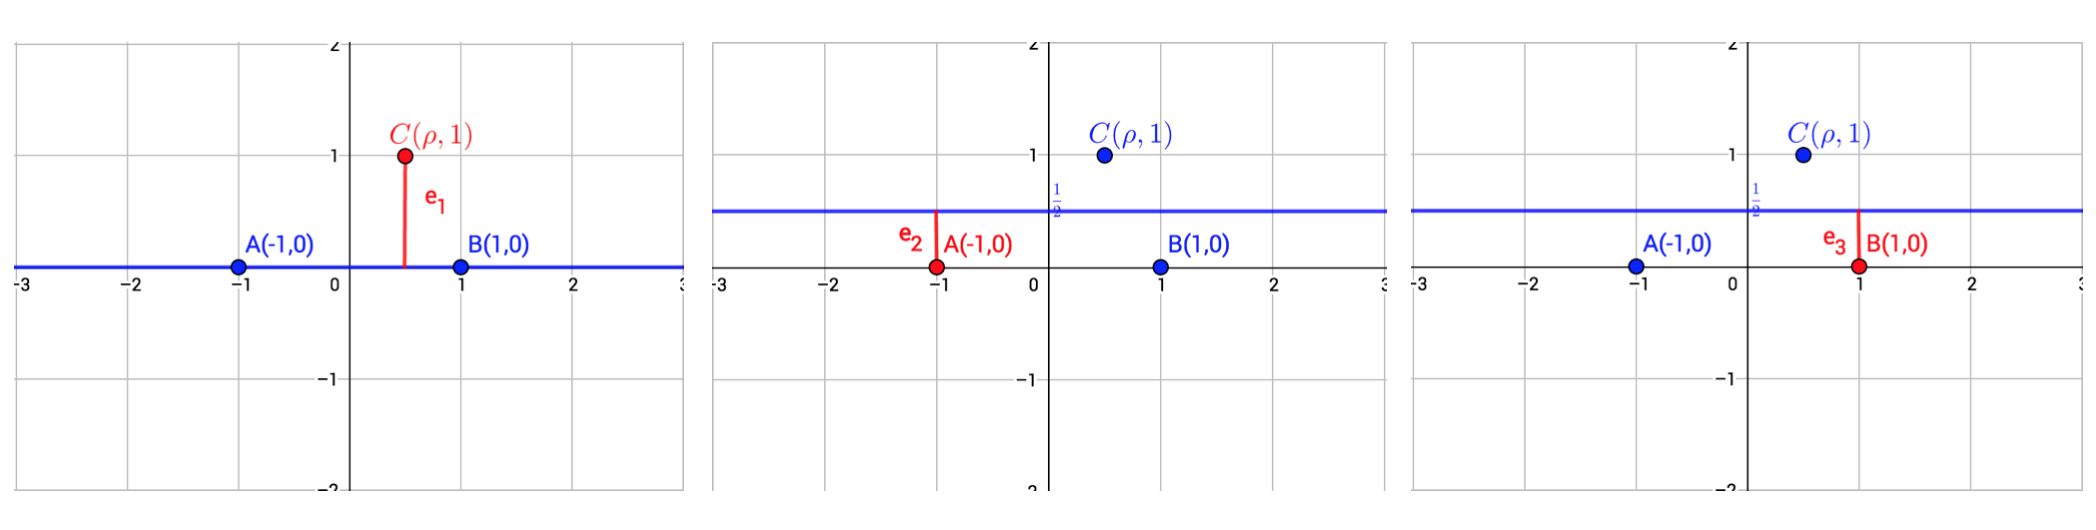
\includegraphics[scale=0.48]{Q41.png}
\end{figure}
 $\displaystyle \therefore E_{loocv}(h_{0})=\frac{1}{3} \cdot (1^2 + (\frac{1}{2})^2 + (\frac{1}{2})^2)= \frac{1}{2}$ \\

\begin{figure}[h]
\centering
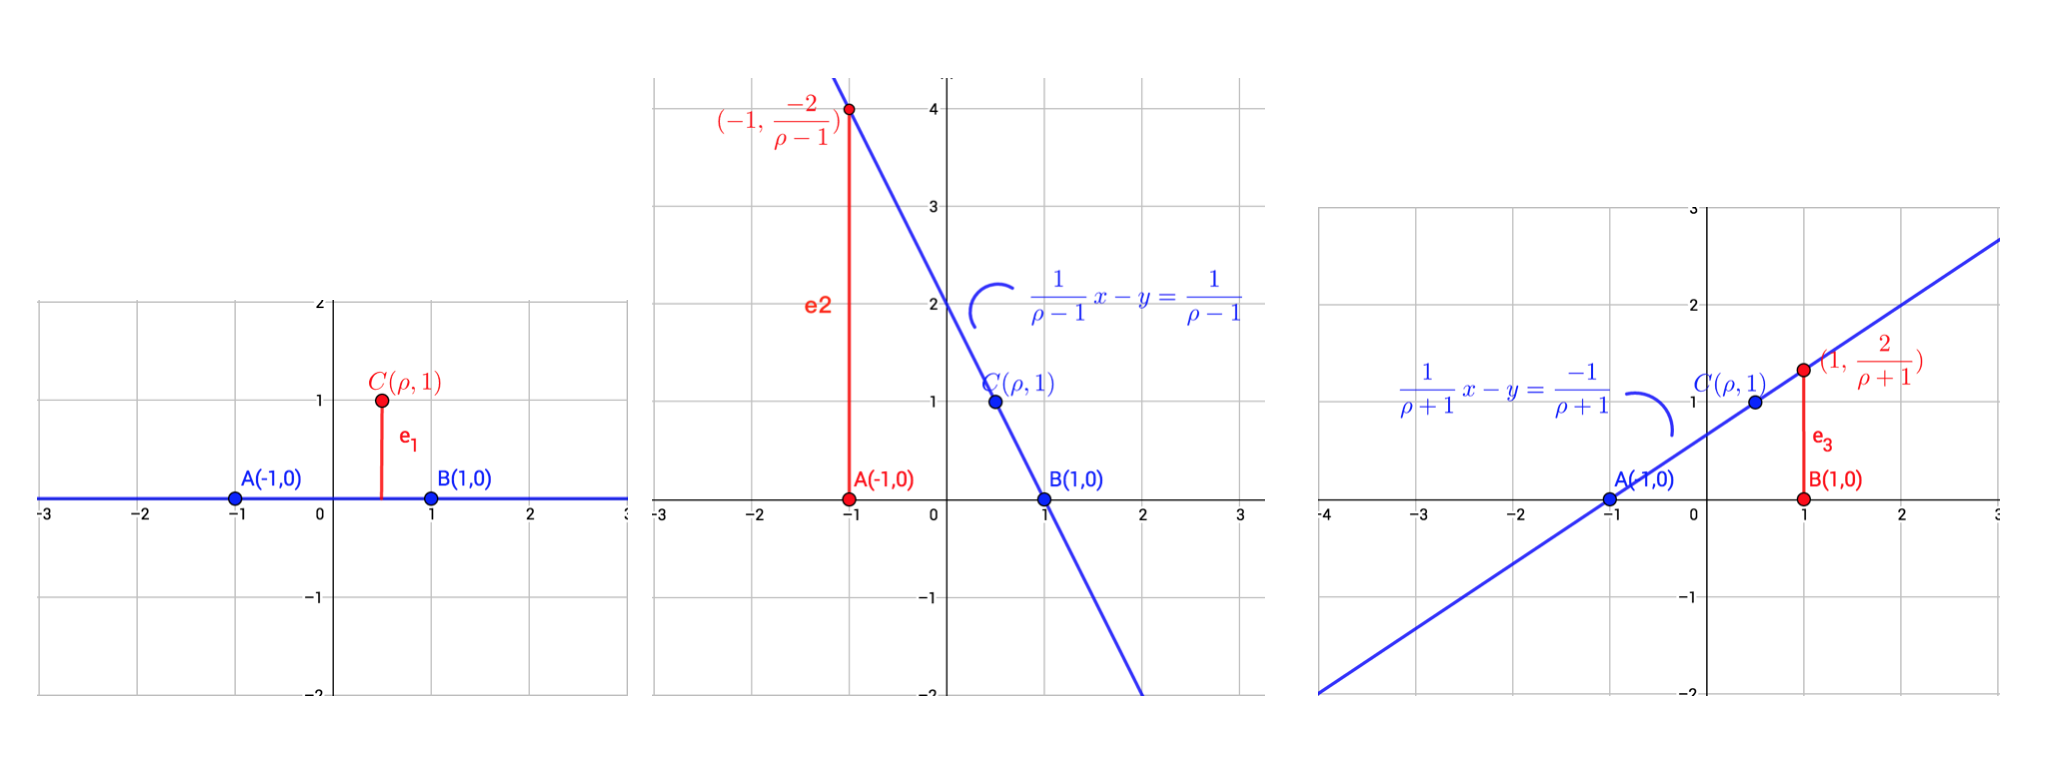
\includegraphics[scale=0.48]{Q42.png}
\end{figure}
 $\displaystyle \therefore E_{loocv}(h_{1})=\frac{1}{3} \cdot (1^2 + (\frac{-2}{\rho-1})^2 + (\frac{2}{\rho+1})^2)$ \\
 \newline
 Let $\displaystyle E_{loocv}(h_{0})=E_{loocv}(h_{1}) \Rightarrow \quad \rho=\sqrt{9+4 \sqrt{6}}$




\section{}
$\displaystyle E_{in}= \frac{1}{N+K} (\mathbf{  wx^Txw - 2w^Tx^Ty + y^Ty + w \widetilde{x}^{T} \widetilde{x} w -2 \widetilde{w}^{T} \widetilde{x} \widetilde{y} + \widetilde{y}^{T} \widetilde{y}      } )$ \\
$\therefore$ $\displaystyle \nabla E_{in} (\mathbf{w})=\frac{1}{N+K} (\mathbf{x^Txw - x^Ty + \widetilde{x}^{T} \widetilde{x} w - \widetilde{x}^{T} \widetilde{y}    })$ \\
F.O.C. $\nabla E_{in}(\mathbf{w})=0 \quad \Rightarrow \mathbf{ w^{*} = (x^Tx + \widetilde{x}^{T} \widetilde{x} )^{-1} (x^Ty +\widetilde{x}^{T} \widetilde{y})   }$.


\section{}
The condition of $\mathbf{w}_{reg}$ given in question is exact the Regularized Regression Problem.\\
By P.10 in slides 14, we know the optimal solution of regularized regression is :
\begin{align*} 
  \mathbf{ w_{reg}^{*} = (x^Tx + \lambda I)^{-1} x^Ty  }
\end{align*}
$\therefore$ Let $\mathbf{ \widetilde{x} = \sqrt{\lambda} I }$, $\mathbf{   \widetilde{y}= 0}$ then $\mathbf{ w^{*}=w_{reg}^{*} }$.



\section{}
  \begin{minipage}{\linewidth}
      \begin{minipage}{0.6\linewidth}
\raggedright
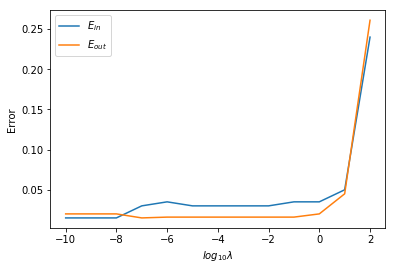
\includegraphics[scale=0.7]{Q7.png}
      \end{minipage}
      \hspace{0.05\linewidth}
      \begin{minipage}{0.4\linewidth}
          In the left figure, we can observe that if we minimize $E_{in}$ by choosing $log_{10} \lambda = 10$,  then $E_{in}$ is close enough to $E_{out}$. This result corresponds to the learning goal: $E_{in} \approx E_{out}$ and $E_{in}, E_{out}$ are small enough.
      \end{minipage}
  \end{minipage}


\section{}
  \begin{minipage}{\linewidth}
      \begin{minipage}{0.6\linewidth}
\raggedright
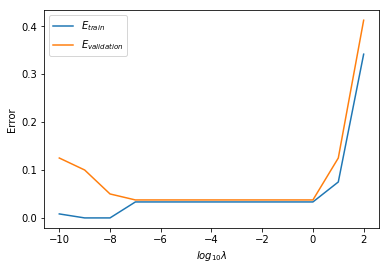
\includegraphics[scale=0.7]{Q8.png}
      \end{minipage}
      \hspace{0.05\linewidth}
      \begin{minipage}{0.4\linewidth}
         We can observer the $E_{validation} \leq E_{train}, \forall \, log_{10} \lambda$. It is quite intuitive since we split the original into two parts "$train$ \& $validation$" and tune the parameter to minimize the error in $train$. The model on $train$ is tend to fit on the training set, the error on $validation$ tend to be higher consequently.
      \end{minipage}
  \end{minipage}

\newpage
\section{}
\begin{itemize}
 \item [(a).] $\displaystyle E_{loocv}= \frac{1}{N} \cdot (e_{1}+e_{2}+ \cdots +e_{N})$, where $N=1126+1126=2252$ \\
  Suppose we select the validation instances "$x_{1}:+, x_{2}:+, \cdots, x_{1126}:+$" corresponding to "$e_{1}, e_{2}, \cdots, e_{1126}$" ; and select the validation instances "$x_{1127}:-, x_{1128}:-, \cdots, x_{2252}:-$" corresponding to "$e_{1127}, e_{1128}, \cdots, e_{2252}$". \\
  \newline
  $\mathcal{A}_{majority}$: Always predicts the majority class.
  \begin{itemize}
   \item [$e_{1}$:] 1 instance with + as validation; 2251 instances as train: $\begin{cases}
1125 \, \text{with} \, + \\
1126 \, \text{with} \, - \Rightarrow \text{Majority}
\end{cases}$\\
   $\therefore e_{1}=1$. Similarly, $e_{2}=e_{3}= \cdots =e_{1126}=1$
   
   \item [$e_{1127}$:] 1 instance with - as validation; 2251 instances as train: $\begin{cases}
1126 \, \text{with} \, + \Rightarrow \text{Majority} \\
1125 \, \text{with} \, - 
\end{cases}$\\
   $\therefore e_{1127}=1$. Similarly, $e_{1128}=e_{1129}= \cdots =e_{2252}=1$
  \end{itemize}
  Hence, $E_{loocv}(\mathcal{A}_{majority})= \frac{1}{2252} \cdot (1+1+ \cdots +1)=\frac{1}{2252}\cdot(2252)=1$\\
 \newline
 $\mathcal{A}_{minority}$: Always predicts the minority class.
  \begin{itemize}
   \item [$e_{1}$:] 1 instance with + as validation; 2251 instances as train: $\begin{cases}
1125 \, \text{with} \, + \Rightarrow \text{minority} \\
1126 \, \text{with} \, - \
\end{cases}$\\
   $\therefore e_{1}=0$. Similarly, $e_{2}=e_{3}= \cdots =e_{1126}=0$
   
   \item [$e_{1127}$:] 1 instance with - as validation; 2251 instances as train: $\begin{cases}
1126 \, \text{with} \, +  \\
1125 \, \text{with} \, - \Rightarrow \text{minority}
\end{cases}$\\
   $\therefore e_{1127}=0$. Similarly, $e_{1128}=e_{1129}= \cdots =e_{2252}=0$
  \end{itemize}
  Hence, $E_{loocv}(\mathcal{A}_{minority})= \frac{1}{2252} \cdot (0+0+ \cdots +0)=\frac{1}{2252}\cdot(0)=0$\\
  Therefore, we will choose $\mathcal{A}_{minority}$ based on $E_{loocv}$.

 \item [(b).] We follow the same strategy of selecting instances as validation in (a). Suppose we have the instances $\left \{ y_{1}, y_{2}, \cdots y_{N} \right \}$, let $\displaystyle \bar{y}=\sum_{i=1}^{N} \frac{y_{i}}{N}$.\\
 \newline
 $\displaystyle e_{1}= \left (y_{1} - \frac{y_{2}+y_{3}+...+y_{N}}{N-1}  \right )^{2} = \left [   y_{1} - \frac{\left ( \bar{y} \cdot N - y_{1} \right )}{N-1} \right ]^{2} = \left (   \frac{y_{1} \cdot N -y_{1}- \bar{y} \cdot N + y_{1}}{N-1} \right )^{2} = \left [    \frac{N\left ( y_{1}- \bar{y} \right )}{N-1}   \right ]^{2}$.\\
 $\displaystyle e_{2}= \left (y_{2} - \frac{y_{1}+y_{3}+y_{4}+...+y_{N}}{N-1}  \right )^{2} = \left [   y_{2} - \frac{\left ( \bar{y} \cdot N - y_{2} \right )}{N-1} \right ]^{2} = \left [    \frac{N\left ( y_{2}- \bar{y} \right )}{N-1}   \right ]^{2}$.\\
 $\vdots$\\
 $\displaystyle e_{N}= \left [    \frac{N\left ( y_{N}- \bar{y} \right )}{N-1}   \right ]^{2}$.\\
 \newline
 Therefore,
 \begin{align*}
  E_{loocv} &= \frac{1}{N} \cdot (e_{1}+e_{2}+...+e_{N}) \\
  &= \frac{1}{N} \cdot \left \{  (\frac{N}{N-1})^{2} \left [  (y_{1}- \bar{y})^2 +  (y_{2}- \bar{y})^2 + ... +  (y_{N}- \bar{y})^2  \right ]   \right \} \\
  &= (\frac{N}{N-1})^2 \cdot \frac{1}{N} \sum_{i=1}^{N} (y_{i}- \bar{y})^2 = (\frac{N}{N-1})^2 \cdot Var(y_{n})
 \end{align*}
 $\therefore$ the scale factor is $\displaystyle (\frac{N}{N-1})^2$
\end{itemize} 




\medskip



\end{document}
